% diversity_reduction_abridged.tex
%
% A short (target: 5-7 pages) self-contained summary of the theory and
% experiments. The full treatment is in diversity_reduction_walkthrough.tex
% (29 pages); this is the "what would I read in 10 minutes" version.
%
% This is wrapper-local material: it re-states the key equations and
% findings in compressed form rather than importing from the modular
% theory files. For the derivations, proofs, and per-claim detail, cross
% references point to the long version.
%
% Required packages: amsmath, amssymb, booktabs, graphicx, hyperref
%                    (no theorem environments; this file only uses
%                     \begin{align*}, \begin{equation}, etc.)
%
% Citation keys: same as the long version (turntrout2023steering,
% turntrout2023norms, mardia2000directional, sinii2025small).


\section{Diversity Reduction in Activation Steering --- Short Version}
\label{sec:abridged}

\paragraph{The question.}
\emph{Activation steering}~\citep{turntrout2023steering} adds a fixed
vector $s \in \mathbb{R}^d$ to a transformer's residual stream at chosen
layers to bias behaviour without retraining. Practitioners observe that
as $\|s\|$ grows, outputs become not just biased but \emph{narrow} --- the
same phrasings, the same answer, repeated. We ask why.

\paragraph{The answer in one sentence.}
Every transformer has normalization layers (RMSNorm / LayerNorm) that project
the residual stream onto a sphere of fixed radius. Adding a fixed offset
before this projection \emph{must} concentrate the post-normalization
distribution toward the pole $\hat{s} = s/\|s\|$; the concentration
tightens as $\|s\|$ grows.

\subsection{Setup}

Let $x \in \mathbb{R}^d$ be a residual-stream activation with
$\mu = \mathbb{E}[x]$ and $\Sigma_x = \operatorname{Cov}(x)$. Let $s$ be
the steering vector, $m = \mu + s$, $\hat{m} = m / \|m\|$. RMSNorm acts as
$v \mapsto v / \|v\|$ up to a learned gain, so we analyze the bare
sphere projection
\[
  g(v) = v / \|v\|, \qquad
  \phi_s(x) = \widehat{x + s}.
\]
The \emph{spherical variance}
$V = 1 - \|\mathbb{E}[\phi_s(x)]\| \in [0,1]$~\citep{mardia2000directional}
is our main summary: $V = 0$ means all outputs project to the same point on
the sphere; $V$ close to $1$ means they are essentially uniform.

\subsection{The Math in Four Lines}

One elementary lemma drives everything. For any nonzero $u, v$,
\begin{equation}
  \|\hat{u} - \hat{v}\| \;\le\; \frac{2\,\|u - v\|}{\max(\|u\|, \|v\|)}.
  \label{eq:ab-chordal}
\end{equation}
Setting $u = x+s,\ v = s$ gives the global \textbf{geometric bound}:
every post-steering point lies in a spherical cap of radius
$2\|x\|/\|s\|$ around the pole $\hat{s}$. Distribution-level bounds
follow by expectation:
\begin{equation}
  V \;\le\; \frac{2\,\mathbb{E}[\|x\|]}{\|s\|}, \qquad
  \operatorname{diam}(\phi_s(\mathcal{D})) \;\le\; \frac{4R}{\|s\|},
  \label{eq:ab-global}
\end{equation}
where $R = \sup \|x\|$. These are exact, distribution-free, and scale as
$O(1/\|s\|)$.

Taylor-expanding $g$ around $m$ to first order (with $\delta = x - \mu$)
gives the local \textbf{covariance bound}:
\begin{equation}
  \Sigma_z \;\approx\; \frac{P_{\perp m}\,\Sigma_x\,P_{\perp m}}{\|m\|^2},
  \qquad
  \operatorname{tr}(\Sigma_z) \;=\; \frac{\operatorname{tr}\Sigma_x - \hat{m}^\top\Sigma_x\hat{m}}{\|m\|^2},
  \label{eq:ab-local}
\end{equation}
where $P_{\perp m} = I - \hat{m}\hat{m}^\top$. Two effects: the projector
$P_{\perp m}$ annihilates the $\hat{m}$ direction (rank drops by 1 when
$\hat{m}^\top\Sigma_x\hat{m} > 0$), and the surviving variation is
rescaled by $1/\|m\|^2$ --- the strong-steering regime shrinks variance
as $O(1/\|s\|^2)$.

The second-order Taylor expansion (sphere curvature) refines the
spherical variance itself:
\begin{equation}
  V \;\approx\; \frac{\operatorname{tr}\Sigma_x - \hat{m}^\top\Sigma_x\hat{m}}{2\,\|m\|^2},
  \qquad
  \|m(s)\|^2 = s^2 \|v_{\mathrm{eff}}\|^2 + 2 s (v_{\mathrm{eff}} \cdot \mu) + \|\mu\|^2.
  \label{eq:ab-second-order}
\end{equation}
The denominator is a \emph{quadratic} in $s$ with floor $\|\mu\|^2$, so
$V(s)$ on a log--log plot is a smooth curve --- flat shelf at
$s \ll \|\mu\|/\|v_{\mathrm{eff}}\|$, slope $-2$ tail at
$s \gg \|\mu\|/\|v_{\mathrm{eff}}\|$ --- not a straight line. This is
the ``parabola on log--log'' we observe empirically.

One side condition: the bounds correspond to a \emph{reduction} relative
to the unsteered baseline only when
\begin{equation}
  \|\mu + s\| > \|\mu\| \;\iff\; \cos\angle(\mu, s) > -\frac{\|s\|}{2\|\mu\|}.
  \label{eq:ab-gate}
\end{equation}
The gate \eqref{eq:ab-gate} is algebraic; it fails only for steering
vectors mildly anti-aligned with the evaluation distribution's residual
mean. This matters in practice (see below).

\subsection{Experiments}

We test on two open-weight models --- Qwen2.5-1.5B-Instruct ($d=1536$)
and Meta-Llama-3-8B-Instruct ($d=4096$), both RMSNorm + RoPE. Input
distribution: $1000$ documents from \texttt{fineweb-edu}, truncated to
$256$ tokens. Steering vectors: three publicly trained vectors from
EasySteer (\texttt{happy}, \texttt{style} for Qwen; \texttt{create} for
Llama), plus two random-direction controls --- \emph{per-layer-matched}
($\|r_\ell\| = \|s_\ell\|$ per layer) and \emph{aggregate-matched}
($\|\sum_\ell r_\ell\| = \|\sum_\ell s_\ell\|$ across target layers).

$19$ recording runs total across scales $c \in \{0, 0.5, 1, 2, 4, 8\}$.
Each run streams $1000$ prompts, intervenes via \texttt{nnsight} at
target layers, and accumulates a $d \times d$ streaming covariance
(hand-rolled Chan--Golub--LeVeque Welford) plus a $K = 1024$ activation
reservoir at the final RMSNorm site.

\subsection{Headline Findings}

\begin{enumerate}
  \item \textbf{The exact geometric bounds always hold.}
    Claim 3 ($\max \|\phi_s(x) - \hat{s}\| \le 2\|x\|/\|s\|$), Claim 5
    (spherical diameter $\le 4R/\|s\|$), Claims 2 and 6 (spherical
    variance and expected pairwise distance $\le 2\mathbb{E}\|x\|/\|s\|$,
    $4\mathbb{E}\|x\|/\|s\|$) pass on every run at every scale. These are
    the pipeline smoke test.

  \item \textbf{Claim 4 is always inapplicable.}
    The pairwise Lipschitz bound requires $\|s\| > R$. Both models have
    $R \approx 10^3$ at the final RMSNorm site while the largest
    $\|s_{\mathrm{eff}}\|$ we could push through is $\approx 120$. The
    precondition is never satisfied.

  \item \textbf{Asymptotic $1/\|s\|$ scaling (Claim 8) manifests on Llama,
    not on Qwen.} Log--log regression slopes for $V(s)$:

    \begin{center}
    \small
    \begin{tabular}{@{}lrr@{}}
      \toprule
      Run & slope $V$ & slope $\operatorname{tr}(\Sigma_z)$ \\
      \midrule
      Llama + \texttt{creativity} (trained) & $\mathbf{-1.92}$ & $-1.77$ \\
      Llama + aggregate-matched random & $\mathbf{-1.85}$ & $-1.71$ \\
      Llama + per-layer-matched random & $-0.51$ & $-0.41$ \\
      Qwen + \texttt{style} & $-0.29$ & $-0.25$ \\
      Qwen + aggregate-matched random & $-0.20$ & $-0.17$ \\
      Qwen + \texttt{happy} & $-0.02$ & $-0.02$ \\
      \bottomrule
    \end{tabular}
    \end{center}

    Llama at $c=4,8$ reaches the regime $\|s_{\mathrm{eff}}\| \gg \|\mu\|$;
    Qwen never does because Qwen's unsteered $\|\mu\| \approx 218$ is too
    large to be dominated by any tolerable steering magnitude.

  \item \textbf{Aggregate magnitude, not semantic direction, drives the
    scaling.} The trained-vs-aggregate-matched-random gap on Llama is
    $0.07$ on slope $V$ --- regression noise. The apparent
    ``trained vectors are special'' effect from Experiment~1 alone
    (trained $-1.92$, \emph{per-layer}-matched random $-0.51$) was an
    artifact of per-layer matching: $n$ near-orthogonal random unit
    vectors stack to $\sqrt{n}$ in aggregate, whereas coherently trained
    vectors stack to $n$. Matching aggregates equates the stacking and
    erases the gap. \textbf{Implication for practice:}
    random-direction baselines should be aggregate-matched, not
    per-layer-matched.

  \item \textbf{The reduction gate (Claim 7) is a precondition, not a
    theorem.} Qwen + \texttt{happy} fails Claim 7 at every scale:
    $\cos(\mu_{\mathrm{unsteered}}, \sum_\ell s_\ell^{\mathrm{happy}}) = -0.108$
    on FineWeb-Edu (educational prose sits slightly on the ``sad'' side
    of the happy-vs-sad axis). Single-layer Qwen interventions at layers
    17 and 25 fail for \emph{both} real and random directions --- a
    direction-independent, position-dependent effect driven by how
    little downstream amplification late-layer interventions receive.
    \textbf{Implication for practice:} verify \eqref{eq:ab-gate}
    empirically on the evaluation distribution before trusting any of
    the bounds on a new $(\text{model}, \text{vector}, \text{dataset})$
    triple.

  \item \textbf{The second-order theory predicts --- and the data confirms ---
    the exact shape of $V(s)$.} Fitting $\|m(s)\|^2 = a s^2 + b s + c$
    on measured $s > 0$ data and extrapolating to $s = 0$ recovers the
    independently-measured $\|\mu\|$:

    \begin{center}
    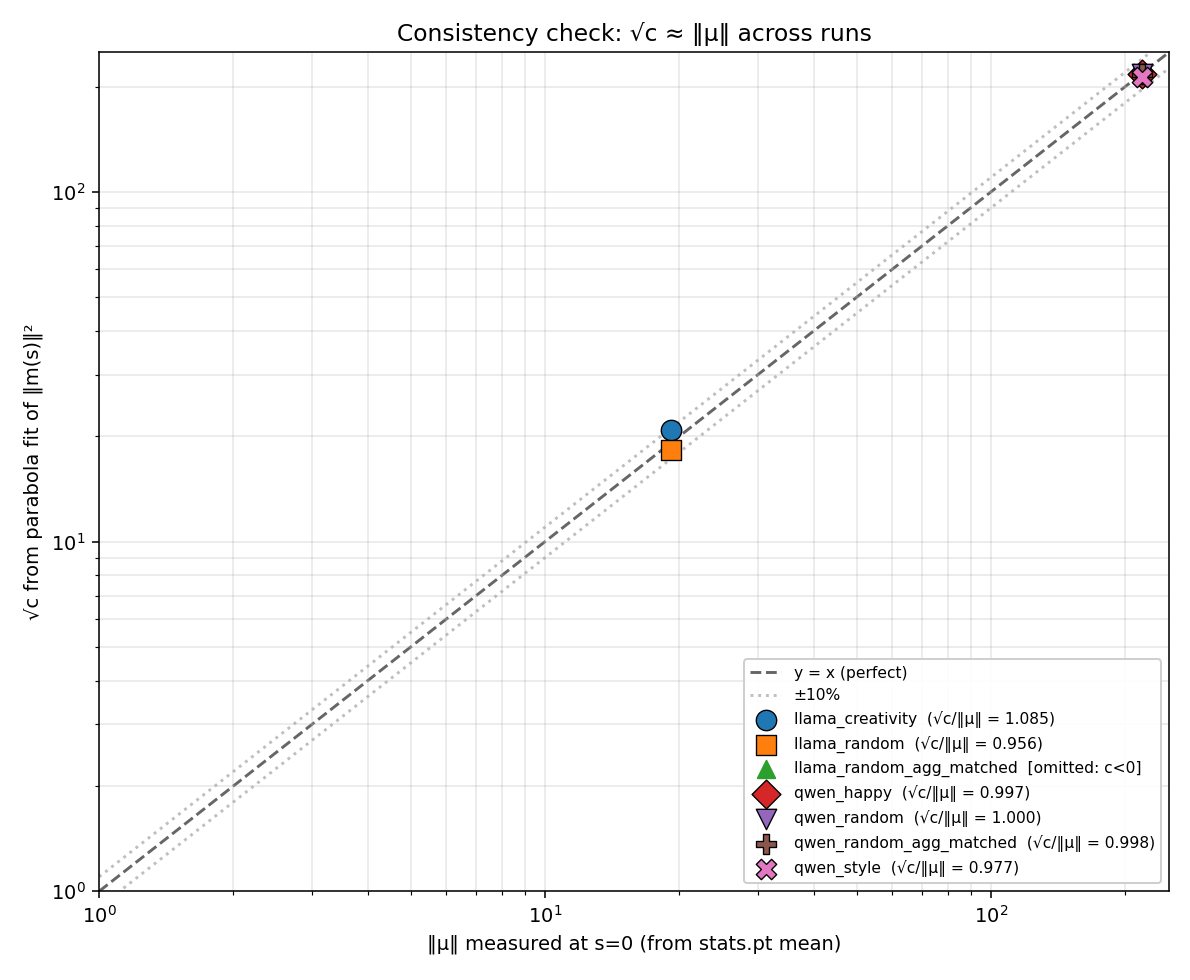
\includegraphics[width=0.72\linewidth]{figures/second_order_overview.png}
    \end{center}

    Six of seven multi-layer runs land within $\pm 10\%$ of the
    $y = x$ diagonal. \texttt{qwen\_random} matches to four decimal
    places. The log--log parabola of $V(s)$ is not a failure of the
    slope-$-1$ prediction; it is a theorem: the second-order formula
    \eqref{eq:ab-second-order} has a quadratic denominator with floor
    $\|\mu\|^2$, and we can \emph{recover} $\|\mu\|$ from the curvature.

  \item \textbf{Claim 9 (eigenalignment) is not observed.} The predicted
    alignment between the smallest eigenvector of $\Sigma_z$ and
    $\hat{m}$ does not manifest at the final-RMSNorm site. Most likely
    cause is that the relevant axis is propagated and rotated relative
    to the injection direction; future work should evaluate at the
    injection layer.
\end{enumerate}

\subsection{Threats to Validity}

\begin{itemize}
  \item A silent batch-indexing bug contaminated the first run
    (HuggingFace Transformers $\ge 4.40$: Qwen2/Llama3 decoder layers
    return a bare tensor, not a tuple; \texttt{.output[0]} indexes the
    batch dimension instead of unpacking). All contaminated results
    are preserved under \texttt{discarded/} for audit; all numbers
    reported above are post-fix.
  \item \texttt{welford-torch} loses $>100\%$ accuracy in the
    big-mean / small-batch regime; the pipeline uses a hand-rolled
    Chan--Golub--LeVeque merge instead. Reproducer filed upstream.
  \item Qwen + \texttt{happy}'s Claim 7 failure is driven by a small but
    systematic training-pool-vs-evaluation-distribution mismatch. Not a
    flaw in the theory; a precondition for it to apply.
\end{itemize}

\subsection{What to Take Away}

The exact geometric bounds \eqref{eq:ab-global} hold unconditionally. The
asymptotic scaling law of Claim 8 and the rank-reducing local covariance
\eqref{eq:ab-local} hold as predicted, but are quantitatively tight only
when aggregate steering magnitude exceeds the natural residual-stream
scale --- a regime Llama-3-8B can reach but Qwen-1.5B cannot within
tolerable output quality. The scaling law is a statement about
\emph{aggregate magnitude}, not semantic direction; future empirical
work should use aggregate-matched random baselines.

The second-order refinement \eqref{eq:ab-second-order} predicts the
log--log parabolic shape of $V(s)$ and lets us recover the unsteered
$\|\mu\|$ from curvature alone, to within $\pm 10\%$ across every run
where the quadratic model is valid.

For full derivations, proofs, per-claim empirical detail, and threats
to validity, see the full walk-through:
\texttt{docs/paper\_sections/diversity\_reduction\_walkthrough.tex}
(29 pages, rendered at
\texttt{docs/paper\_sections/build/diversity\_reduction\_walkthrough.pdf}).

Code, configs, and per-run outputs are at
\url{https://github.com/AMindToThink/steering_diversity} under
\texttt{src/bounds/}, \texttt{scripts/bounds/}, and
\texttt{outputs/bounds/}.
